Muitos problemas reais de controle ótimo apresentam um controle limitado, dado
que em geral o controle indica uma medida a ser tomada e ela possui limitações
práticas. Por exemplo, se o controle for a quantidade de um químico, no
Laboratório 3 do Capítulo \ref{labs123}, não podemos adicionar uma quantidade
negativa desse químico, o que nos leva a restringir $u(t) \ge 0$ e também não
temos uma quantidade infinita do químico disponível e talvez seja tão limitada
que devemos impor $u(t) \le C$. 

\section{Condições Necessárias} 

Considere o problema
\begin{gather*}
    \max_u J(u) = \max_u \int_{t_0}^{t_1} f(t,x(t),u(t))dt + \phi(x(t_1)) \\
    \text{sujeito a   }x'(t) = g(t,x(t),u(t)), x(t_0) = x_0, \\
    a \leq u(t) \leq b, a < b
\end{gather*}

Seja $u^*$ e $x^*$ o par ótimo. Seja $h(t)$ uma função contínua por partes tal
que exista $\e_0$, de forma que $\forall \e \in (0,\e_0], u^{\e}(t) = u^*(t) +
\e h(t)$ é admissível sob os limites inferior e superior. Devido aos limites,
o funcional pode não ser zero no controle ótimo, dado que esse pode estar nos
limites. Seja $x^{\e}(t)$ a variável do estado correspondente. Da mesma forma
que fizemos no capítulo \ref{ch:1}, seja $\la(t)$ uma função diferenciável por
partes e, assim 
\begin{multline}
    \label{eq:8-1}
    J(u^{\e}) = \int_{t_0}^{t_1} \left[f(t,x^{\e}, u^{\e}) + \la(t)g(t,x^{\e}, u^{\e}) + x^{\e}\la '(t)\right]dt \\
    - \la(t_0)x_0 + \la(t_1)x^{\e}(t_1) + \phi(x(t_1))
\end{multline}    

Como $J(u^*)$ é máximo, temos que 
\begin{equation}
    \label{eq:8-2}
    0 \ge \frac{d}{d\e}J(u^{\e})\bigg\vert_{\e = 0} = \lim_{\e \to 0^+} \frac{J(u^{\e}) - J(u^*)}{\e}
\end{equation}

Como já fizemos, tome a variável $\la(t)$ de forma que 
$$
\la '(t) = -[f_x(t,x^*, u^*) + \la(t)g_x(t,x^*,u^*)], \la(t_1) = \phi '(x^*(t_1))
$$
Então \refeq{eq:8-1} e \refeq{eq:8-2} se reduzem a 
$$
0 \ge \int_{t_0}^{t_1} (f_u + \la g_u)h dt,
$$
E essa desigualdade vale para toda função $h$. Seja $s$ um ponto de
continuidade tal que $a \le u^*(s) < b$. Suponha que $f_u + \la g_u > 0$ em
$s$. Pela continuidade de $u^*$ em $s$, vale que $f_u + \la g_u$ é contínua em
$s$ e, portanto, deve ser positiva em uma vizinhança do ponto. Podemos tomar esse
intervalo menor para que tenhamos $u^* < b$. Seja $I$ o maior intervalo
fechado com essas características e defina  
$$
M = \max\{u^*(t): t \in I\}
$$
Seja 
$$
h(t) = \begin{cases}
    b - M > 0, &\text{se }t \in I, \\
    0,     &\text{se }t \not\in I
\end{cases}
$$
Portanto $a \le u^* + \e h \le b$ quando $\e \in [0,1]$. Mas
$$
\int_{t_0}^{t_1} (f_u + \la g_u)h dt = \int_I (f_u + \la g_u)(b-M) dt > 0,
$$
uma contradição. Portanto $f_u + \la g_u \le 0$. 

De forma similar, se $s$ é um ponto onde $u^*$ é contínua e $a < u^*(s) \le
b$, teremos que em $s$, $f_u + \la g_u \ge 0$. E assim, 
\begin{align*}
    u^*(t) = a &\implies f_u + \la g_u \le 0 \text{ em } t, \\
    a < u^*(t) < b &\implies f_u + \la g_u = 0 \text{ em } t, \\
    u^*(t) = b &\implies f_u + \la g_u \ge 0 \text{ em } t, 
\end{align*}

De forma equivalente 
\begin{align}
    \label{eq:8-3}
    f_u + \la g_u > 0 \text{ em } t &\implies u^*(t) \neq a , \\
    \label{eq:8-4}
    f_u + \la g_u \neq 0 \text{ em } t  &\implies u^*(t)=a \text{ ou } u^*(t)=b, \\
    \label{eq:8-5}
    f_u + \la g_u < 0 \text{ em } t &\implies u^*(t) \neq b, 
\end{align}

De \refeq{eq:8-3} e \refeq{eq:8-4}, vemos que $f_u + \la g_u > 0 \implies
u^*(t) = b$. De \refeq{eq:8-4} e \refeq{eq:8-5}, vemos que $f_u + \la g_u < 0
\implies u^*(t) = a$. E, por fim, se $f_u + \la g_u = 0 \implies a \le u^*(t)
\le b$. Para os pontos em que $u^*$ não é contínua, não precisamos nos
preocupar, pois não afetam o funcional objetivo. Portanto, temos que, dado o
Hamiltoniano $H$, 
\begin{gather*}
    x'(t) = \frac{\partial H}{\partial \la}, x(t_0) = x_0 \\ 
    \la '(t) = - \frac{\partial H}{\partial x}, \la(t_1) = \phi '(x(t_1)) \\
    \begin{cases}
        u^* = a &\text{ se } H_u < 0 \\
        a \le u^* \le b &\text{ se } H_u = 0 \\
        u^* = b &\text{ se } H_u > 0 \\
    \end{cases}
\end{gather*}

Em um problema de minimização, as desigualdades da primeira e terceira linhas
são revertidas. A condições de transversalidade são todas equivalentes ao caso
não limitado, isto é, a dualidade do estado e adjunta é a mesma. 

\section{Soluções Numéricas}

Uma mudança no algoritmo é necessária para calcular a solução numérica.  As
equações estado e adjunta não são alteradas, pois não dependem dos limites de
$u^*$ e apenas a sua caracterização.  Além disso, o chute inicial deve ser
entre os limites do controle. As mudanças necessárias podem ser visualizadas na seção de exemplos. 

\section{Exemplos}

\begin{example}
    \begin{gather*}
        \max_u x(4) - \int_0^4 u(t)^2 dt \\ 
        \text{sujeito a  }x'(t) = x(t) + u(t), x(0) = 0, \\
        u(t) \le 5
    \end{gather*}
\end{example}

O Hamiltoniano é dado por $H = -u^2 + \la x + \la u$. A equação adjunta é
dada por 
$$
\la '(t) = -H_x = -\la \implies \la(t) = Ke^{-t}
$$
Como $\la(4) = \phi '(x^*(4)) = 1$, temos que $Ke^{-4} = 1 \implies K =
e^4$. Assim $$\la(t) = e^{4 - t}.$$
Além disso, $H_u = -2u + \la$. Como o controle não tem limite inferior,
temos que $H_u < 0$ não pode ocorrer. 

Se $H_u > 0 \implies u^{*}(t) = 5 \implies \lambda - 10 > 0 \implies e^{4
- t} > 10 \implies t < 4 - \log 10$

Se $H_u = 0 \implies u^*(t) = \frac{1}{2}e^{4-t} \le 5$. Portanto $t \ge 4
- \log 10$. 

Consequentemente, 
$$
u^* = \begin{cases}
    5 &\text{quando } 0 \le t < 4 -\log 10 \\
    \frac{1}{2}e^{4-t} &\text{quando } 4 - \log 10 \le t \le 4
\end{cases}
$$

Agora vamos encontrar o estado associado. 

$$
x'(t) = x(t) + 5 \implies x(t) = 5e^t - 5, t \in [0, 4-\log 10]
$$
$$
x'(t) = x(t) + \frac{1}{2}e^{4-t} \implies x(t) = -\frac{1}{4}e^{4-t} + ke^t, t \in [4 - \log 10, 4]
$$
para alguma constante $k$ de forma que $x^*$ seja contínua, isto é, as
expressões concordem. Isso ocorre quando $k = 5 - 25e^{-4}$. 

\begin{example}
    Considere o simples exemplo 
    \begin{gather*}
        \min_u \int_0^4 u(t)^2 + x(t) dt \\ 
        \text{sujeito a  }x'(t) = u(t), x(0) = 0, x(4) = 1 \\
        u(t) \ge 0 
    \end{gather*}
\end{example}

Vamos visualizar a diferença entre a solução com limites e sem limites. Para
problemas com limites, é importante que não apenas trunquemos o resultado. 

No exemplo, o Hamiltoniano é dado por $H = \la_0(u^2 + x) + \la u$. A função adjunta
é dada por 
$$\la '(t) = - H_x = -\la_0 \implies \la(t) = k - \la_0 t, 
$$
para alguma constante $k$ e $\la_0 = 0 \text{ ou } \la_0 = 1$. 
A condição de otimalidade é 
$$
H_u = 2\la_0 u + \la, 
$$
$$
H_u > 0 \implies u^*(t) = 0 \implies 0 < \la = k - t \implies t < k,
$$
Considere $\la_0 = 1$.
$$
H_u = 0 \implies 0 \le u^*(t) = -\frac{\la}{2} = \frac{t-k}{2} \implies t \ge k
$$
Portanto 
$$
u^*(t) = \begin{cases}
    0, &\text{ quando } 0 \le t < k, \\ 
    \frac{t-k}{2} &\text{ quando } k \le t \le 4
\end{cases}
$$
Agora precisamos encontrar o valor de $k$. Para isso, precisamos utilizar as condições de estado inicial e de fronteira. Considere os casos: 

\begin{enumerate}[label=\textbf{Caso \arabic*:}]
    \item $k \le 0$. Assim $x'(t) = u = \frac{t - k}{2} \implies x(t) = \frac{t^2}{4} - \frac{kt}{2} + c$, tal que $c=0$ e $x(4) = 4 - 2k = 1 \implies k = 3/2$, um absurdo. 
    
    \item $k \ge 4$. Assim $u^* \equiv 0$. Então $x^* \equiv c$, o que também é um absurdo. 
    
    \item Então $0 < k < 4$. Nesse caso $x'(t) = 0 \implies x \equiv c = 0$ em $[0,k)$. Em $[k,4], x'(t) = \frac{t-k}{2}$ e, portanto, 
    $$
    x(t) = \frac{t^2}{4} - \frac{kt}{2} + c,
    $$
    para alguma constante $c$. Pela continuidade de $x$, $c = \frac{k^2}{4}$, pois $x(k) = 0$. Por fim, $1 = x(4) = 4 - 2k + k^2/4$. A solução é portanto $k = 2 \text{ ou } 6$. Como $k < 4 \implies k = 2$. Concluímos então que 
\end{enumerate}
$$
u^*(t) = \begin{cases}
    0, &\text{ quando } 0 \le t < 2, \\ 
    \frac{t-2}{2} &\text{ quando } 2 \le t \le 4
\end{cases} \text{ e } x^*(t) = \begin{cases}
    0, &\text{ quando } 0 \le t < 2, \\ 
    \frac{(t-2)^2}{4} &\text{ quando } 2 \le t \le 4
\end{cases}
$$

Agora, vamos procurar o controle ótimo $\hat{u}$ sem restrição. Nesse caso 
$$
\hat{u}(t) = \frac{t-k}{2} \implies \hat{x}(t) = \frac{t^2}{4} - \frac{kt}{2}
+ c
$$
tal que $x(0) = c = 0$ e $x(4) = 4 - 2k = 1 \implies k = 3/2$. Assim, se só truncássemos a solução, teríamos 
$$
\hat{u}(t) = \begin{cases}
    0, &\text{ quando } 0 \le t < 3/2, \\ 
    \frac{2t-3}{4} &\text{ quando } 3/2 \le t \le 4
\end{cases}
$$

Em conclusão, para encontrar controle ótimo com restrição, devemos considerá-los nas contas. 

\begin{figure}[!hb]
    \center
    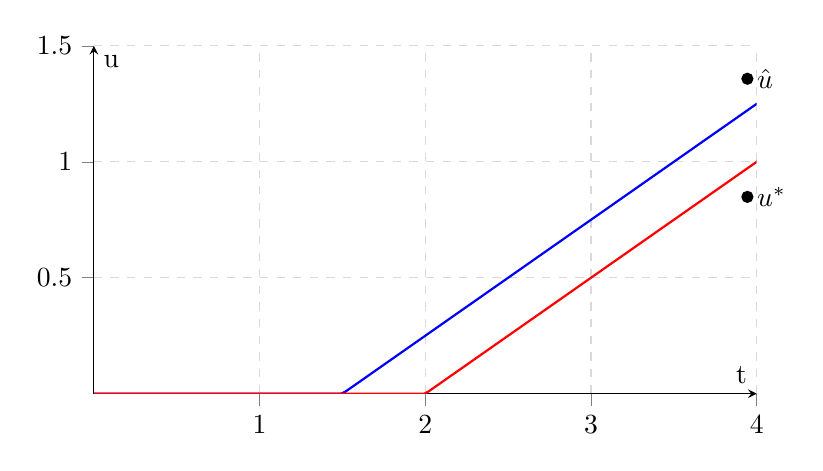
\begin{tikzpicture}[
    declare function={
        f(\x)= (\x <= 1.5) * (0)   +
                  (\x >= 1.5) * (0.5*\x - 0.75)
       ;
       g(\x) =  (\x <=  2) * (0)   +
                  (\x >= 2) * (0.5*\x - 1) 
       ;
      }
    ]
    \begin{axis}[
        axis x line=middle,
        axis y line=middle,
        grid = major,
        width=10cm,
        height=6cm,
        grid style={dashed, gray!30},
        xmin= 0,     % start the diagram at this x-coordinate
        xmax= 4,    % end   the diagram at this x-coordinate
        ymin= 0,     % start the diagram at this y-coordinate
        ymax= 1.5,   % end   the diagram at this y-coordinate
        xlabel=t,
        ylabel=u,
		/pgfplots/xtick={0, 1, ..., 4}, % make steps of length 0.5
		/pgfplots/ytick={0, 0.5, ..., 4}, % make steps of length 0.5
        tick align=outside,
        samples = 400,
        enlargelimits=false]
      % plot the function
	  \addplot [blue,thick] {f(x)};
	  \addplot [red,thick] {g(x)};
    \end{axis}

    \filldraw[black] (8.3,2.5) circle (2pt) node[anchor=west] {$u^*$};
    \filldraw[black] (8.3,4.0) circle (2pt) node[anchor=west] {$\hat{u}$};

\end{tikzpicture}
    \caption{Controles ótimo e com truncagem}
\end{figure}